% This is a sample content just for reference

\section{Introduction}

This is how you reference pictures in the text: (Figure ~\ref{fig:figure1}) \\
This is how you cite: \cite[Some page, some paraghaph]{hawking1988} \\
This is how you create nice tables, and reference them (See table ~\ref{table:tab1})

\begin{table}[ht]
    \captionof{table}{Assets selected for portfolio}
    \label{table:tab1}
    \begin{tabular}{@{}rrrrrr@{}}
    \toprule
    \textbf{Ticker} & \textbf{Company name}      & \boldmath{$\beta$} & \textbf{Sector}        & \textbf{Industry}  \\ 
    \midrule
    WMT       & Walmart Inc.            & 0.507262      & Consumer Defensive     & Discount Stores                  \\
    XOM       & Exxon Mobil Corporation & 0.936712      & Energy                 & Oil \& Gas Integrated               \\
    TSLA      & Tesla, Inc.             & 1.43901       & Consumer Cyclical      & Auto Manufacturers                \\
    NEM       & Newmont Corporation     & 0.292796      & Basic Materials        & Gold                                \\
    KR        & Kroger Company (The)    & 0.311054      & Consumer Defensive     & Grocery Stores                      \\
    GIS       & General Mills, Inc.     & 0.379007      & Consumer Defensive     & Packaged Foods                       \\
    META      & Meta Platforms, Inc.    & 1.201507      & Communication Services & Internet Content \& Information     \\
    MRNA      & Moderna, Inc.           & 0.456853      & Healthcare             & Biotechnology                     \\ 
    \bottomrule
    \end{tabular}
\end{table}

\begin{figure}[ht]
    \begin{center}
        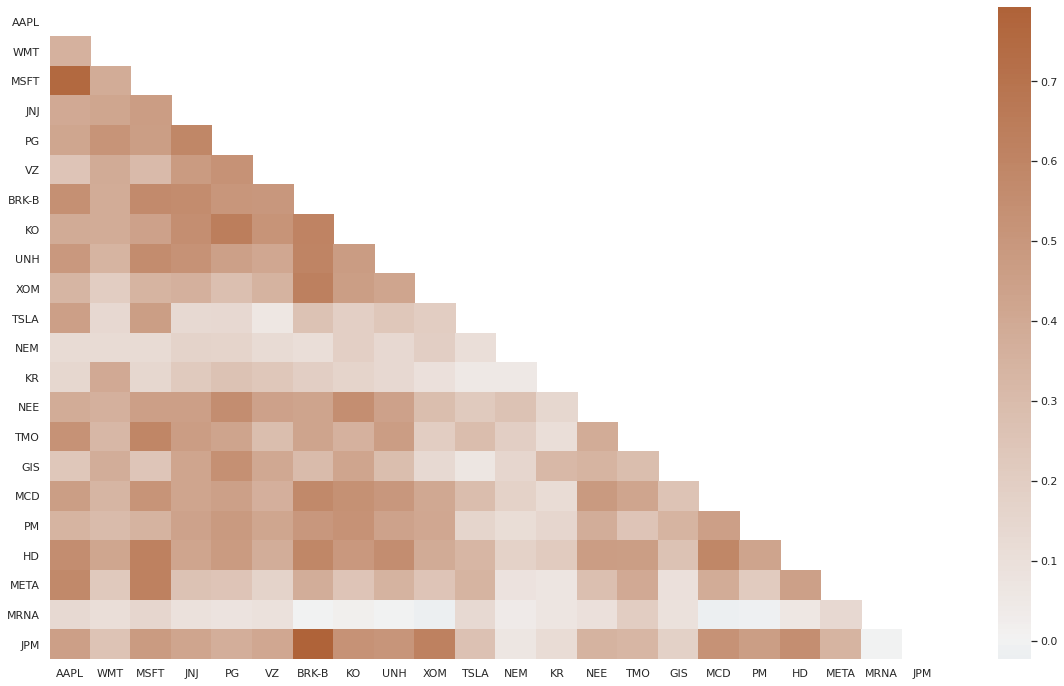
\includegraphics[width=0.8\textwidth]{img/fig1.png}
        \caption{Picture description}
        \label{fig:figure1}
    \end{center}
\end{figure}

This is how you do math and reference equations (\ref{eq:1}):

\begin{equation} \label{eq:1}
    w^*=\frac{\Sigma^{-1}(\mu_{BL}-r_f\mathbf{1})}{\mathbf{1}^T\Sigma^{-1}(\mu_{BL}-r_f\mathbf{1})}   
\end{equation}

$$
E = mC^2
$$

This is how you inline math: 
$\quad \dfrac{\partial L}{\partial \omega}(\omega, \lambda, \gamma) = \omega'\Sigma - \lambda\mu' - \gamma\mathbf{1}' = 0 \quad$ 
in the normal text

This is how you do bullet lists:

\begin{itemize}
    \item Item 1
    \item Item 2
    \item Item 3
\end{itemize}

Or numbered lists:

\begin{enumerate}
    \item Item
    \item Item
    \item Item
\end{enumerate}

\noindent
New paragraph with no indent. New paragraph with no indent. New paragraph with no indent. New paragraph with no indent. New paragraph with no indent. New paragraph with no indent. New paragraph with no indent.

Paragraph with indent. Paragraph with indent. Paragraph with indent. Paragraph with indent. Paragraph with indent. Paragraph with indent. Paragraph with indent. Paragraph with indent. Paragraph with indent. Paragraph with indent.


\newpage
\section{Methods}
\section{Research Body}
\subsection{Very Important Topic 1}
\subsubsection{Item 1}
\subsubsection{Item 2}
\subsubsection{Item 3}
\newpage
\subsection{Very Important Topic 2}
\newpage
\section{Conclusion}